\section{Experiments}

\subsection{Experimental Setup}\label{sec:setup}
We first evaluate \toolName{} on two representative benchmarks that stress complementary aspects of multi-agent coordination: software-engineering test-time scaling and long-context multi-doc reasoning. Section~\ref{sec:with_rlm} later studies how \toolName{} can be combined with RLM~\citep{zhang2025recursive}.

(1) \textbf{SWE-bench Verified}~\citep{jimenez2024swebench}. A software-engineering benchmark built from real-world GitHub issues with human-verified task specifications and tests. We use it to evaluate agentic coding in realistic repository environments, where agents must inspect codebases, identify relevant files, implement fixes, and validate them through tests. This benchmark is especially suitable for our setting because its tasks require iterative exploration and coordination over large codebases rather than retrieving a single local answer.

(2) \textbf{LongBench-v2}~\citep{bai2025longbench}. A long-context benchmark designed to evaluate deep understanding and reasoning over realistic tasks. We focus on its multi-document QA setting, which contains 125 samples across diverse domains: Financial (15 samples), Government (23 samples), Multi-News (23 samples), Legal (14 samples), and Academic (50 samples). This setting is also suitable for our evaluation because its questions require multi-hop reasoning over evidence distributed across long contexts, rather than extracting a single local span.


We compare \toolName{} against different baselines. 
\textbf{Base} directly invokes the LLM once over the full input to produce an answer, without any decomposition or multi-agent orchestration. 
\textbf{Claude Code}~\citep{anthropic_claude_code_2026} is a tool-augmented agentic baseline that performs programmatic inspection and context compression to handle long inputs. \textbf{mini-SWE-agent}~\citep{yang2024sweagent} is a lightweight software-engineering agent that uses a simple linear agent loop with Bash as its primary interface.
\textbf{AOrchestra}~\citep{ruan2026aorchestra} is a centralized multi-agent system in which a main orchestrator dynamically creates specialized sub-agents on demand, instantiating each as a tuple of instruction, context, tools, and model to execute individual subtasks. 
\textbf{ReadAgent}~\citep{lee2024human} is an agentic long-context baseline that compresses the input into short gist memories and looks up the original passages when a subtask needs details the gists omit. For base models, we use Gemini 3 Flash~\citep{doshi2025gemini3flash} and Claude Opus 4.6~\citep{anthropic2026opus46} for the SWE-bench experiments; and GPT-5.4~\citep{openai2026gpt54}, Claude Sonnet 4.6~\citep{anthropic2025claude46sonnet}, Gemini 3 Flash, and DeepSeek-V4-Pro~\citep{deepseekai2026deepseekv4} for the LongBench-v2 experiments. 

All base models are evaluated through OpenRouter with default reasoning and sampling parameters. For Claude Code, we route the CLI through OpenRouter to support alternative base models and allow access to tools such as Read, Grep, and Bash. For AOrchestra, following the original configuration, we set \texttt{max-attempts = 10} for the orchestrator and \texttt{max-steps = 50} for each sub-agent. For ReadAgent, we set \texttt{min-lookup-pages = 1} and \texttt{max-lookup-pages = 6}, and use a 100-token gist budget, matching the gist budget used by \toolName{}.

\subsection{SWE-bench Verified}
\label{sec:swe}
SWE-bench Verified evaluates whether \toolName{} can improve test-time scaling in agentic software-engineering tasks. These tasks are largely sequential: each action depends on the outcome of the previous one, leaving little room to parallelize work {within} a single trajectory. Therefore, we scale {across} trajectories: we run each task $X$ times (with $X\in\{2,4\}$) and count it as solved if any one of the $X$ attempts yields a correct patch. We report three metrics: \textbf{Avg.@1} is the mean per-trial success rate, i.e., the expected accuracy of a single attempt; while \textbf{Pass@2} and \textbf{Pass@4} measure whether at least one of 2 or 4 attempts solves the task. 

Different methods use the same test-time scaling budget in different ways. For Base, mini-SWE-agent, Claude Code, and the original AOrchestra, we run $X$ independent attempts per task. Each trajectory starts from scratch and does not reuse intermediate discoveries from other attempts. We also introduce AOrchestra-Parallel, a variant built on AOrchestra. It starts each task once, but allows the main agent at each step to spawn up to $X$ subtasks and sub-agents in parallel, aggregate their outputs, and use the combined information to decide the next step. These parallel threads are therefore coupled through the main agent. \toolName{} uses the same agent harness as AOrchestra and likewise allows parallel threads to inform one another, but agents communicate through a verified shared context rather than through a central controller.
\begin{table}[t]
\centering
\setlength{\tabcolsep}{8pt}
\renewcommand{\arraystretch}{1.15}
\caption{Comparison on SWE-bench Verified across two base models. Best values are bolded.}
\label{tab:swebench_verified}
\begin{threeparttable}
\begin{tabular}{@{}l ccc | c@{}}
\toprule
\textbf{Method} & \textbf{Avg.@1} & \textbf{Pass@2} & \textbf{Pass@4} & \textbf{Cost/Task} \\
\midrule
\multicolumn{5}{@{}l}{\textit{Gemini 3 Flash}}\\
mini-SWE-agent       & 54.7\% & 65.6\% & 75.1\% & \$0.26 \\
Claude Code          & 49.3\% & 57.1\% & 66.3\% & --\,\tnote{a}    \\
AOrchestra           & 55.2\% & 64.5\% & 73.2\% & \$0.24 \\
AOrchestra-Parallel  & 56.4\% & 63.2\% & 71.8\% & \$0.25 \\
\rowcolor{rowgray}\textbf{\toolName{}} & \textbf{65.7\%} & \textbf{72.9\%} & \textbf{77.4\%} & \textbf{\$0.12} \\
\midrule
\multicolumn{5}{@{}l}{\textit{Claude Opus 4.6}}\\
mini-SWE-agent       & 76.9\% & 79.8\% & 81.7\% & \textbf{\$0.61} \\
Claude Code          & 76.1\% & 79.5\% & 81.3\% & \$0.69   \\
AOrchestra           & 74.7\% & 78.3\% & 80.1\% & \$0.70 \\
AOrchestra-Parallel  & 75.2\% & 78.1\% & 79.7\% & \$0.73 \\
\rowcolor{rowgray}\textbf{\toolName{}} & \textbf{78.0\%} & \textbf{80.7\%} & \textbf{82.5\%} & \$0.63 \\
\bottomrule
\end{tabular}
\begin{tablenotes}[flush]
\footnotesize
\item[a] The Claude Code CLI sends \texttt{cache\_control} blocks in the Anthropic API format, so cache reuse only works if the upstream provider honors those blocks. For Gemini-3-Flash the real cost without cache reuse is therefore around \$1 per task.
\end{tablenotes}
\end{threeparttable}
\end{table}

Table~\ref{tab:swebench_verified} shows that \toolName{} achieves the best performance across both base models. With Gemini 3 Flash, \toolName{} reaches 65.7\% Avg.@1, 72.9\% Pass@2, and 77.4\% Pass@4, outperforming all baselines on every metric. The largest gain appears in Avg.@1, where \toolName{} exceeds the strongest baseline, AOrchestra-Parallel, by 9.3 percentage points. At the same time, \toolName{} reduces cost to \$0.12 per task, roughly half the cost of the strongest agentic baselines. This shows that the improvement comes from using the same test-time budget more effectively, rather than from launching more trajectories or spending more tokens.

AOrchestra-Parallel improves Avg.@1 over the original AOrchestra, but performs worse on Pass@2 and Pass@4. This suggests that coupling parallel threads through a main agent can make attempts more consistent, but may also reduce exploration diversity.

The gains with Claude Opus 4.6 are smaller, likely because the base model is already strong and leaves less room for coordination to help. Even so, \toolName{} still achieves the highest accuracy across Avg.@1, Pass@2, and Pass@4, while remaining close to the lowest-cost method, only \$0.02 per task above mini-SWE-agent.

Overall, these results support our central claim: test-time scaling is more effective when parallel agents communicate through shared state. By making compact progress visible across trajectories, \toolName{} lets later agents avoid redundant exploration, build on prior findings, and focus on unresolved parts of the task. Section~\ref{sec:swe_analyze} analyzes these mechanisms through trace-level examples.
\vspace{-7mm}
\subsubsection{Why \toolName{} Is Both Accurate and Cost-Efficient on SWE-bench}
\label{sec:swe_analyze}
\vspace{-2mm}
% takeaway, and reorder
% First, parallel agents complement each other by sharing their failures and facts. Second, admitted constraints remain binding shared state instead of being softened or lost through a central controller. Third, compact patch summaries carry useful discoveries across threads without exposing every worker to long raw traces. 

Three trace-level mechanisms explain why \toolName{} improves both accuracy and cost efficiency. In the \toolName{} traces below, each shared entry is one thread's verified note, tagged with its thread id (\texttt{t0}, \texttt{t1}, \dots) and a type such as \texttt{FACT}, \texttt{FAIL}, or \texttt{PATCH\_SUMMARY}.

\vspace{-2mm}
\paragraph{(1) Parallel agents complement each other by sharing failures.}
The first mechanism is that failed hypotheses become reusable state rather than private dead ends. In isolated forks, a negative result remains local to one trajectory, so other attempts may spend their own budget rediscovering the same failure. In \toolName{}, once such a failure is admitted to the shared context, later agents can treat it as a constraint and redirect their search.

This mechanism appears in the trace below. The task fixes \texttt{lambdify} for single-element tuples. The natural guess, the Python printer layer, is a red herring; the real bug is on a separate tuple-building path in \texttt{sympy/\allowbreak utilities/\allowbreak lambdify.py}:

\begin{lstlisting}[style=gist]
[t0/FACT] AbstractPythonCodePrinter change did not affect lambdify output
[t1/FACT] sympy/utilities/lambdify.py:964 _recursive_to_string manual tuple join bypasses printer fix
[t0/FACT] sympy/utilities/lambdify.py:964 manual join for tuples lacks trailing comma logic
\end{lstlisting}
 
The load-bearing update is the negative result in the first line: thread \texttt{t0} shows that changing the printer does not affect the output. After reading this failure, \texttt{t1} avoids repeating the same detour and localizes the actual bypass in \texttt{\_recursive\_to\_string}; \texttt{t0} then records the concrete defect, the missing trailing comma. Thus, \toolName{} turns a failed hypothesis into shared progress, improving later agents' search efficiency.

\vspace{-2mm}
\paragraph{(2) Admitted constraints remain binding shared state.}
The second mechanism is that \toolName{} preserves important constraints as
shared state rather than routing them through a central controller. In centralized coordination, a main agent may soften, omit, or reopen constraints discovered by sub-agents before they can guide later work.
 
This mechanism appears in the trace below. Folding multiple search filters into one \texttt{.filter()} call is unsafe for multi-valued relations, where \texttt{.filter(A).\allowbreak filter(B)} and \texttt{.filter(A, B)} differ. In AOrchestra-Parallel, a sub-agent finds exactly this danger, but the constraint must pass through the main agent, which reopens the optimization and softens it into a tradeoff about reducing joins ``for many use cases''; the run fails. The relevant fact was found, but not preserved as binding state. In contrast, \toolName{} keeps the constraint explicit and reusable:
 
\begin{lstlisting}[style=gist]
[t3/FAIL] django/contrib/admin/options.py:1041 single .filter() breaks M2M multi-term search
[t3/FACT] Django ORM .filter(Q1, Q2) vs .filter(Q1).filter(Q2) differs for multi-valued relations
[t3/FACT] lookup_spawns_duplicates determines if single .filter() is safe
[t1/FACT] lookup_spawns_duplicates preserves M2M search semantics while optimizing FKs
\end{lstlisting}

Thread \texttt{t3} records the unsafe case (\texttt{FAIL}), the semantic reason, and the predicate \texttt{lookup\_spawns\_duplicates}, which determines when the optimization is valid. Thread \texttt{t1} then builds on this state to preserve M2M semantics while still optimizing foreign-key cases. Thus, later threads inherit the binding constraint rather than reopening a globally invalid simplification.


\paragraph{(3) Compact patch summaries carry discoveries.} 
The third mechanism is compact sharing, which lowers cost by preventing peer
communication from becoming another long raw transcript. Sharing full traces
would preserve information, but would also expose every worker to command
history, file dumps, failed edits, and intermediate reasoning. \toolName{}
instead shares a compressed version of the useful discovery, so later workers can reuse the result without reading the entire trajectory.

This mechanism appears in the trace below. Both the shared and no-share settings solve the task, but compact sharing reduces the cost from \$0.399 to \$0.125. The difference is not that \toolName{} shares more context; rather, it shares a compressed version of the useful search result (labeled as \texttt{PATCH\_SUMMARY}), which is generated by an LLM summarizer. One thread first rules out the ordinary tuple-printer path and localizes the actual bypass in \texttt{lambdify.py}:

\begin{lstlisting}[style=gist]
[t1/FACT] StrPrinter._print_tuple at sympy/printing/str.py:868 already includes trailing comma logic
[t1/FACT] sympy/utilities/lambdify.py:964 lacks trailing comma for single-element tuples
[t1/PATCH_SUMMARY] files=sympy/utilities/lambdify.py | idea=Modify _recursive_to_string to add a trailing comma for single-element tuples | evidence=reproduce_issue.py PASSED
\end{lstlisting}

This patch summary turns a multi-step debugging trajectory into a short,
evidence-backed handoff. Later workers do not need the full command history, file dumps, failed edits, or intermediate reasoning. Thus, compact sharing preserves the reusable discovery while avoiding the cost of exposing every peer to the raw trace, explaining why \toolName{} solves the task at much lower cost.

 
Together, these examples explain the trend in Table~\ref{tab:swebench_verified}: \toolName{} keeps reusable facts, failures, constraints, and patch summaries visible to all peers, while avoiding both redundant isolated search and the high token cost of raw trace sharing. This improves per-thread success while reducing cost.

\subsection{LongBench-v2 Multi-Doc QA}
\label{sec:longbench}
\begin{table}[t]
\centering
\setlength{\tabcolsep}{5pt}
\renewcommand{\arraystretch}{1.2}
\caption{Accuracy (\%) comparison on LongBench-v2 Multi-Doc QA across four base models. Results are mean$\pm$std over 3 independent runs. Numbers in parentheses denote the number of samples in each domain. Best values are bolded.}
\label{tab:multidoc_results}
\begin{tabular}{@{}l ccccc | c@{}}
\toprule
\textbf{Method} & \textbf{Fin.} (15) & \textbf{Govern.} (23) & \textbf{MNews} (23) & \textbf{Legal} (14) & \textbf{Acad.} (50) & \textbf{Avg.} \\
\midrule
\multicolumn{7}{@{}l}{\textit{GPT-5.4}}\\
Base & 62.2\tiny{$\pm$9.3} & 39.1\tiny{$\pm$1.7} & 50.5\tiny{$\pm$8.6} & {62.0}\tiny{$\pm$4.4} & 56.0\tiny{$\pm$1.2} & 53.9\tiny{$\pm$4.9} \\
Claude Code & {65.0}\tiny{$\pm$8.3} & 36.2\tiny{$\pm$2.0} & 50.7\tiny{$\pm$2.0} & 59.5\tiny{$\pm$3.4} & \textbf{60.7}\tiny{$\pm$0.9} & 54.4\tiny{$\pm$3.1} \\
ReadAgent & 
{57.8}\tiny{$\pm$3.9} & 34.8\tiny{$\pm$5.0} & 52.2\tiny{$\pm$8.7} & 
{61.9}\tiny{$\pm$4.4} &
58.0\tiny{$\pm$1.2} &
53.0\tiny{$\pm$3.3} \\
\rowcolor{rowgray}\textbf{\toolName{}} & \textbf{71.1}\tiny{$\pm$3.1} & \textbf{43.5}\tiny{$\pm$2.0} & \textbf{65.2}\tiny{$\pm$2.0} & \textbf{64.3}\tiny{$\pm$5.8} & {56.0}\tiny{$\pm$2.8} & \textbf{60.1}\tiny{$\pm$1.2} \\
\midrule
\multicolumn{7}{@{}l}{\textit{Claude Sonnet 4.6}}\\
Base & 68.9\tiny{$\pm$3.9} & 34.8\tiny{$\pm$1.1} & 46.4\tiny{$\pm$2.0} & 52.4\tiny{$\pm$3.4} & 64.0\tiny{$\pm$0.9} & 53.3\tiny{$\pm$1.9} \\
Claude Code & 66.7\tiny{$\pm$1.1} & 42.0\tiny{$\pm$2.0} & 47.8\tiny{$\pm$4.4} & 50.0\tiny{$\pm$3.4} & 52.0\tiny{$\pm$3.4} & 51.7\tiny{$\pm$2.4} \\
ReadAgent & 62.2\tiny{$\pm$3.9} & {44.9}\tiny{$\pm$4.4} & 43.5\tiny{$\pm$4.4} & 57.1\tiny{$\pm$4.1} & \textbf{64.7}\tiny{$\pm$2.3} & 54.5\tiny{$\pm$3.8} \\
\rowcolor{rowgray}\textbf{\toolName{}} & \textbf{73.3}\tiny{$\pm$3.1} & \textbf{46.4}\tiny{$\pm$2.0} & \textbf{55.1}\tiny{$\pm$2.0} & \textbf{59.5}\tiny{$\pm$3.4} & \textbf{64.7}\tiny{$\pm$0.9} & \textbf{59.8}\tiny{$\pm$1.5} \\
\midrule
\multicolumn{7}{@{}l}{\textit{Gemini 3 Flash}}\\
Base & {80.0}\tiny{$\pm$0.0} & 30.4\tiny{$\pm$0.0} & 43.5\tiny{$\pm$0.0} & \textbf{71.4}\tiny{$\pm$0.0} & 60.0\tiny{$\pm$2.3} & 57.1\tiny{$\pm$3.3} \\
Claude Code & 73.3\tiny{$\pm$3.1} & 26.1\tiny{$\pm$1.5} & 39.1\tiny{$\pm$0.0} & 57.1\tiny{$\pm$2.1} & 52.0\tiny{$\pm$1.9} & 49.5\tiny{$\pm$2.2} \\
ReadAgent & 75.6\tiny{$\pm$2.3} & 21.7\tiny{$\pm$4.4} & 46.4\tiny{$\pm$2.9} & 69.0\tiny{$\pm$3.4} & 62.0\tiny{$\pm$2.3} & 54.9\tiny{$\pm$1.1} \\
\rowcolor{rowgray}\textbf{\toolName{}} & \textbf{82.2}\tiny{$\pm$3.1} & \textbf{37.8}\tiny{$\pm$1.6} & \textbf{52.2}\tiny{$\pm$1.5} & \textbf{71.4}\tiny{$\pm$0.0} & \textbf{64.0}\tiny{$\pm$0.0} & \textbf{61.5}\tiny{$\pm$0.6} \\
\midrule
\multicolumn{7}{@{}l}{\textit{DeepSeek-V4-Pro}}\\
Base & \textbf{86.7}\tiny{$\pm$3.1} & 47.8\tiny{$\pm$2.0} & 44.9\tiny{$\pm$2.0} & \textbf{76.2}\tiny{$\pm$3.4} & 64.0\tiny{$\pm$0.9} & 63.9\tiny{$\pm$1.3} \\
Claude Code & 84.4\tiny{$\pm$3.1} & 36.2\tiny{$\pm$2.0} & 56.5\tiny{$\pm$4.4} & 64.3\tiny{$\pm$2.1} & 48.7\tiny{$\pm$0.9} & 58.0\tiny{$\pm$0.9} \\
ReadAgent & 71.1\tiny{$\pm$3.9} & 43.5\tiny{$\pm$4.4} & 30.4\tiny{$\pm$2.3} & 38.1\tiny{$\pm$4.1} & 50.7\tiny{$\pm$1.2} & 46.8\tiny{$\pm$1.8} \\
\rowcolor{rowgray}\textbf{\toolName{}} & \textbf{86.7}\tiny{$\pm$5.4} & \textbf{52.2}\tiny{$\pm$2.0} & \textbf{59.4}\tiny{$\pm$4.4} & 73.8\tiny{$\pm$3.4} & \textbf{65.3}\tiny{$\pm$0.9} & \textbf{67.5}\tiny{$\pm$1.2} \\
\bottomrule
\end{tabular}
\end{table}
LongBench-v2 Multi-Doc QA evaluates whether \toolName{} can improve evidence aggregation across long documents. Unlike SWE-bench Verified, where progress within one trajectory is largely sequential, this setting exposes substantial within-task parallelism: different agents can inspect different documents, identify complementary evidence, and contribute to a shared answer state.

As shown in Table~\ref{tab:multidoc_results}, \toolName{} achieves the highest average accuracy across all four model families: 60.1\% with GPT-5.4, 59.8\% with Claude Sonnet 4.6, 61.5\% with Gemini 3 Flash, and 67.5\% with DeepSeek-V4-Pro. Compared with the strongest baseline for each model family, these correspond to gains of 5.7, 5.3, 4.4, and 3.6 percentage points, respectively. \toolName{} also achieves the best or tied-best result in most domain-model combinations, suggesting that the benefit comes from a general improvement in evidence selection and reuse rather than from a single model or domain.

These gains come from first building a verified hierarchical view of the document set, enabling more targeted detailed inspection. \toolName{} first splits the input into chunks and uses a lightweight summarizer, DeepSeek-V4-Flash~\citep{deepseekai2026deepseekv4} by default, to produce hierarchical summaries. Verified gists are then admitted to the shared context, giving all agents a compact view of the corpus before they choose what to inspect in detail. This upfront global view helps agents identify cross-document connections, selectively unfold evidence, and avoid poorly targeted reading.

In contrast, centralized and programmatic-inspection baselines make more local inspection decisions, often from metadata, file names, or keyword matches before observing the relevant content. Early mistakes can therefore compound: a controller may inspect the wrong evidence, miss cross-document links, or require additional rounds of delegation. ReadAgent also uses gists, but its lookup process directly depends on lossy summaries, without hierarchical unfolding and admission-time verification. As a result, these baselines can cost less in long-context settings because they avoid the upfront cost of constructing and verifying a structured view of the full context. \toolName{} makes a different trade-off: it spends additional computation on hierarchical summarization and verification, but gains a more reliable understanding of the corpus, leading to more targeted evidence selection and higher prediction accuracy.

% \subsection{LongCoT-mini (Math and CS)}
% LongCoT-mini evaluates a complementary failure mode: rather than aggregating evidence across documents, the model must manage an extended reasoning trajectory that must be decomposed, checked, and recombined. Results are shown in Figure~\ref{fig:cot}. On Gemini-3-Pro, \toolName{} improves over the Base model from 18.0\% to 26.0\% on CS and from 26.3\% to 30.5\% on Math. On GPT-5.2, \toolName{} improves from 40.0\% to 47.0\% on CS and matches the strongest baseline on Math at 30.5\%. 

% These results suggest that the same shared-context construction extends beyond document-level evidence aggregation to intermediate reasoning traces. In this setting, verification is especially important: before an agent trace is summarized into an $G$ entry and admitted to $C$, \toolName{} checks whether its conclusion is well-supported. This prevents wrong local results from becoming shared premises, reducing error propagation across long reasoning trajectories.
% \begin{figure}[!h]
%     \centering
%     \begin{subfigure}{0.48\linewidth}
%         \centering
%         \includegraphics[width=\linewidth]{laa_cot_gemini.pdf}
%         \caption{Gemini-3-Pro Accuracy}
%     \end{subfigure}
%     \hfill
%     \begin{subfigure}{0.48\linewidth}
%         \centering
%         \includegraphics[width=\linewidth]{laa_cot_gpt.pdf}
%         \caption{GPT-5.2 Accuracy}
%     \end{subfigure}
%     \caption{Accuracy on LongCoT-mini for Gemini-3-Pro and GPT-5.2 across the CS and Math domains. \toolName{} achieves the highest accuracy in all four settings, while Claude Code and RLM show inconsistent gains relative to the single-agent base.}
%     \label{fig:cot}
% \end{figure}

% \subsection{Latency and Token Cost}\label{sec:cost}
% Figure~\ref{fig:latency} reports averaged latency and token consumption on the LongBench-v2 multi-document QA task. \toolName{} is slower than the plain Claude Code baseline due to additional overhead from summarization, verification, and shared-state management. However, it is substantially more efficient than RLM: latency decreases from 174.3s to 118.6s, making \toolName{} approximately $1.5\times$ faster, and token consumption decreases from 169K to 111K tokens, making it approximately $1.5\times$ more cost-efficient.

% This gap reflects differences in how context is explored. RLM plans and selects subcontexts based on limited signals, such as metadata or partial observations, before fully reading their content. When early selections are irrelevant or misaligned with the question, subsequent iterations compensate by exploring additional regions of the context, often up to the iteration limit, increasing latency and token usage. In contrast, \toolName{} allows agents to reason over a compact, content-aware representation before selectively unfolding only the necessary details. As a result, its retrieval is more targeted, reducing redundant exploration and improving overall efficiency.
% \begin{figure}[!h]
%     \centering
%     \includegraphics[width=0.99\linewidth]{latency_cost.pdf}
%     \caption{Latency and token consumption on multi-document QA. \toolName{} is $1.5\times$ faster and $1.5\times$ cheaper than RLM, while incurring overhead relative to the simpler Claude Code baseline due to its summarization, verification, and shared-context management.}
%     \label{fig:latency}
% \end{figure}
\vspace{-3mm}
\subsubsection{Which Components Make \toolName{} Effective on LongBench-v2}
\label{sec:longbench_ablation}

\begin{figure}[!h]
    \centering
    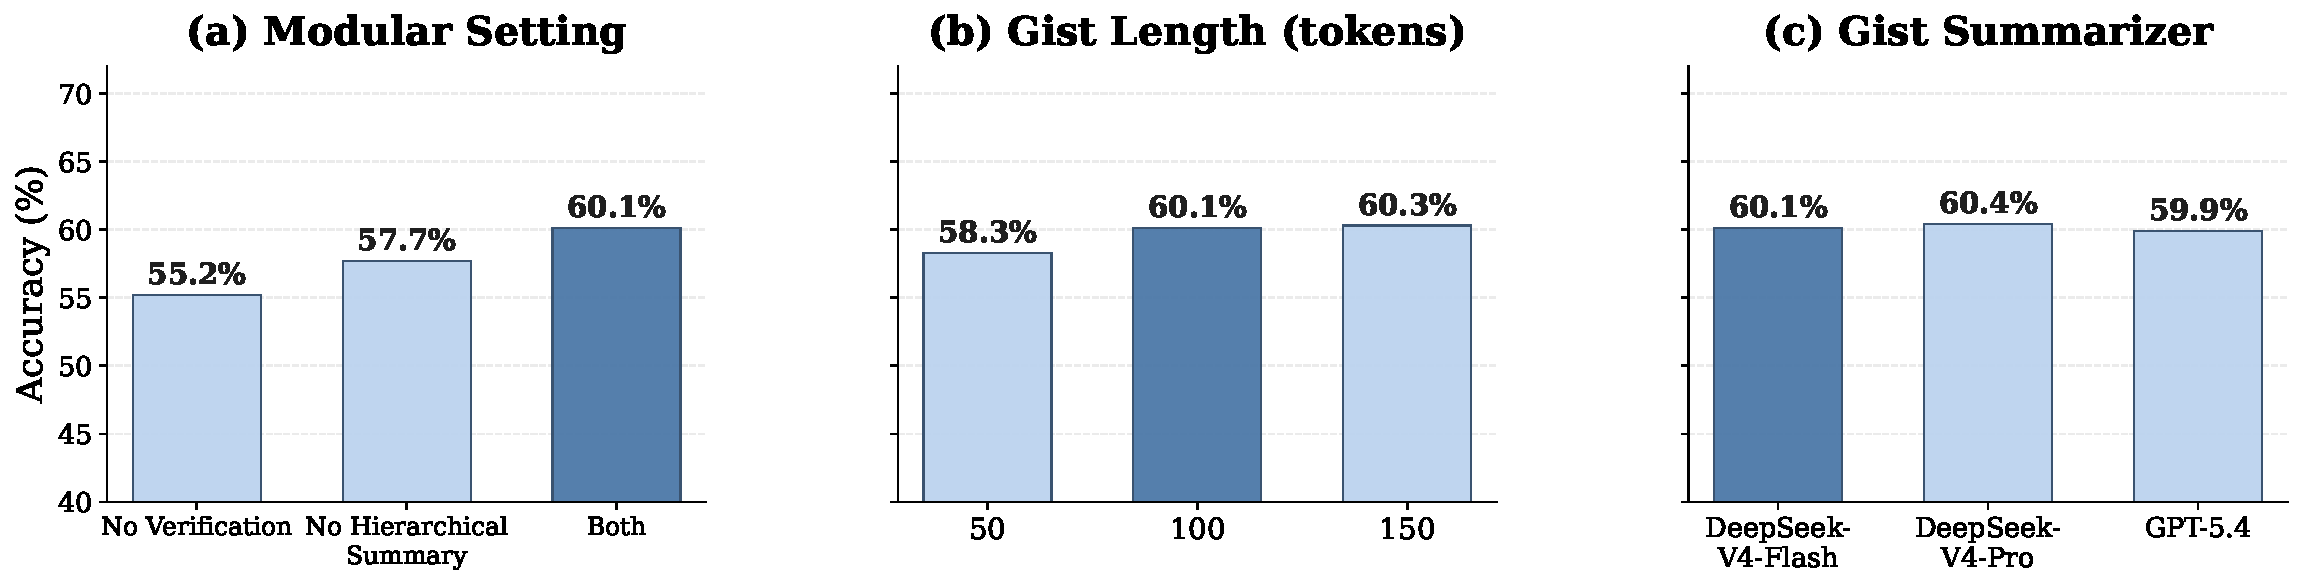
\includegraphics[width=1\linewidth]{ablation.pdf}
    \caption{\textbf{Ablation and robustness analysis on LongBench-v2 Multi-Doc QA.} All bars report accuracy averaged over the five domains with GPT-5.4. (a) Modular ablation: removing either the verification step or the hierarchical summary lowers accuracy. (b, c) \toolName{} is largely insensitive to its gist configuration: accuracy is stable once the gist is long enough (b) and across summarizers of varying cost (c). In every panel, the darker bar marks the default configuration used in Table~\ref{tab:multidoc_results}.}
    \label{fig:ablation}
\end{figure}
% \vspace{-3mm}
\paragraph{Modular ablation.}
To isolate the contribution of \toolName{}'s two core components, we remove admission-time verification and hierarchical summarization in turn, and report average accuracy over the five domains in Figure~\ref{fig:ablation}(a). Removing verification causes the largest drop, from 60.1\% to 55.2\%, showing that unsupported claims can corrupt downstream reasoning when they enter the shared context unchecked. Removing hierarchical summarization also hurts performance, lowering accuracy to 57.7\%, because gist-only routing provides a coarser path from global navigation to raw evidence. Thus, both components matter, with verification contributing the larger gain.

The trajectory evidence explains why the ``No Hierarchical Summary'' ablation degrades performance. Without the intermediate $S_i$ layer, \toolName{} must either route from a lossy gist directly to raw chunks or unfold many raw chunks to recover missing details. The PUMA EBIT query illustrates this failure mode. The document contains competing 2024 EBIT outlooks: an earlier range from the annual report and a later narrowed range from the H1 2024 interim report. The gist layer identifies candidate chunks, but the $S_i$ summary is what determines which source is later in time, localizes the relevant sub-chunk, and flags that the exact EBIT range must be recovered from raw evidence: (\texttt{S72.2} denotes the second segment of chunk 72, retrieved by scanning summary \texttt{S72}.)
\begin{lstlisting}[style=gist]
[t1] The later-in-time source is the H1 2024 interim report, which reiterates sales growth expectations and a narrowed EBIT outlook. The latest 2024 EBIT guidance is located in [S72.2].
[t1] However, the summaries do not provide the actual EBIT range values, so the precise latest target cannot be determined from summaries alone.
\end{lstlisting}

Only after this coarse-to-fine localization does the worker request raw evidence. The deep unfold then retrieves the precise anchored sub-chunk rather than the full report (\texttt{RAW} denotes the corresponding raw text recovered by unfolding):
\begin{lstlisting}[style=gist]
[S72.2 RAW] ... we narrow our outlook for the operating result (EBIT) to a range of EUR 620 million to EUR 670 million ...
\end{lstlisting}

This example shows why the hierarchy $G_i \rightarrow S_i \rightarrow \text{raw}$ is load-bearing. The gist supports cheap global navigation, the $S_i$ summary localizes the relevant raw span and detects when summary-level evidence is insufficient, and raw unfolding recovers the exact values. Removing the $S_i$ layer therefore weakens both evidence localization and cost-controlled reasoning, matching the performance drop in Figure~\ref{fig:ablation}(a).


The trajectory evidence also explains why removing verification hurts performance. In \toolName{}, agent outputs are not admitted into the shared context immediately; they must first be checked against their cited evidence. This prevents plausible but unsupported statements from becoming reusable shared state. In a legal question comparing \textit{Lucy v. Zehmer} and \textit{Texaco v. Pennzoil}, one agent introduced a specific damages claim that was not supported by its cited summary:
\begin{lstlisting}[style=gist]
[t2 OUTPUT] Pennzoil/Texaco is summarized as only conditionally affirmed, with punitive damages reduced from USD 3 billion to USD 1 billion [S5].
\end{lstlisting}
However, the cited gist only states that the case involved a conditional affirmance with remittitur; it does not contain the specific damages amounts. The verifier (an LLM) therefore rejects the update:
\begin{lstlisting}[style=gist]
[t2 VERIFY] WRONG: the claim that punitive damages were reduced from USD 3 billion to USD 1 billion is unsupported;[S5] only says there was a conditional affirmance with remittitur and gives no specific amounts.
\end{lstlisting}
After retry, the unsupported numerical claim is removed before the result is committed to $C$. Without this admission-time gate, the false detail would become available to later workers and the finisher as if it were grounded evidence, explaining the drop under the ``No Verification'' ablation in Figure~\ref{fig:ablation}(a).

\paragraph{Gist length.}
We vary the target gist length across 50, 100, and 150 tokens per source unit (Figure~\ref{fig:ablation}(b)). Accuracy improves from 58.3\% at 50 tokens to 60.1\% at 100 tokens, then plateaus at 60.3\% with 150 tokens. This suggests a threshold effect: once the gist is long enough to capture a source unit's relevance, additional length provides little benefit. We therefore use 100 tokens in the main experiments. Selective unfolding likely contributes to this stability, since agents can recover finer details from $S_i$ or the raw source when the gist is insufficient.

\paragraph{Summarization model.}
We also vary the gist summarizer ($\phi_2$, defined in \S~\ref{sec:summarization}), using DeepSeek-V4-Flash, DeepSeek-V4-Pro, and GPT-5.4 while keeping the rest of the pipeline fixed (Figure~\ref{fig:ablation}(c)). Accuracy remains nearly unchanged across the three summarizers (60.1\%, 60.4\%, and 59.9\%, respectively), with the cheapest model, DeepSeek-V4-Flash (our default), matching the stronger alternatives. Thus, a lightweight summarizer is sufficient for constructing the shared context, allowing \toolName{} to reserve stronger models for subtask reasoning without sacrificing accuracy.

\section{Combining \toolName{} with RLM}\label{sec:with_rlm}
Recursive Language Models (RLMs)~\citep{zhang2025recursive} process long contexts by recursively selecting context segments, issuing sub-calls, and composing the resulting partial answers. Crucially, RLM performs this process through a code-mediated Read-Eval-Print Loop (REPL): the long input is stored as an external variable that the model can inspect, parse, and aggregate programmatically. This makes RLM a natural fit for OOLONG~\citep{bertsch2025oolong}, an aggregation-heavy benchmark where each sample consists of timestamped, user-attributed entries and answering a question often requires classifying many entries before computing a distributional answer.

\begin{wraptable}{r}{0.5\textwidth}
\centering
\begin{tabular}{lcc}
\toprule
\textbf{Method} & \textbf{Acc.} & \textbf{Cost/Task} \\
\midrule
\multicolumn{3}{l}{\textit{OOLONG}} \\
RLM & 56.0\% & \$0.43 \\
\toolName{} & 53.3\% & \$0.47 \\
\toolName{}+RLM & \textbf{64.0\%} & \textbf{\$0.40} \\
\midrule
\multicolumn{3}{l}{\textit{LongBench-v2 Multi-Doc QA}} \\
RLM & 55.8\% & \$0.29 \\
\toolName{} & 57.9\% & \$0.30 \\
\toolName{}+RLM & \textbf{60.3\%} & \textbf{\$0.24} \\
\bottomrule
\end{tabular}
\caption{Comparison of RLM, \toolName{}, and their hybrid on LongBench-v2 Multi-Doc QA and OOLONG using GPT-5.}
\label{tab:oolong}
\end{wraptable}

We first evaluate \toolName{} and RLM separately on both LongBench-v2 Multi-Doc QA and OOLONG using GPT-5 with medium reasoning (RLM uses GPT-5-mini for sub-calls and recursion depth=1). As shown in Table~\ref{tab:oolong}, the two methods have complementary strengths. On LongBench-v2, \toolName{} achieves higher average accuracy than RLM at roughly the same cost per task. On OOLONG, however, \toolName{} underperforms RLM in both average accuracy and cost. This is because OOLONG is closer to a structured data-processing benchmark than a conversational reasoning benchmark (such as LongBench-v2): many questions require exact counting, filtering, comparison, and tie handling. In this setting, the natural-language shared context used by \toolName{} is not reliable. RLM performs better because its core interface is code-mediated: through a REPL environment, the model can inspect, parse, transform, and aggregate the input using executable programs and programmatic sub-calls. However, RLM still relies on centralized coordination, where recursive calls report back to a root process that must reconcile and aggregate their outputs. This centralized aggregation is less suitable for natural-language multi-document reasoning, helping explain RLM's weaker LongBench-v2 performance. These results motivate a hybrid design that combines RLM's precise REPL-based execution with \toolName{}'s decentralized coordination.

We therefore combine the two methods by retaining RLM as the underlying reasoner while adding two \toolName{} components: a verified shared context and a decentralized task queue. In this hybrid setting, there is no main-agent/sub-agent hierarchy; all agents are equally ranked RLM instances that coordinate through shared state. An initial RLM call produces a compact work plan, after which subtasks are placed into the task queue and claimed by parallel RLM workers. Each worker's output is admitted into the shared context only after passing the verification gate. The system then generates any additional subtasks from the current problem state, and computes the final answer from the verified shared context once no further subtasks are needed. This design preserves RLM's strength in precise code-mediated execution while adding \toolName{}'s decentralized coordination. As shown in Table~\ref{tab:oolong}, the combined method achieves the best accuracy and lowest cost on both benchmarks, indicating that RLM and \toolName{} are complementary rather than competing approaches.